\documentclass{beamer}
\usepackage[english,french]{babel}
\usepackage[T1]{fontenc}
\usepackage[utf8]{inputenc}
\usepackage[math]{kurier}

\usepackage{graphicx, color, subfigure, wrapfig, afterpage, fancyhdr,
  graphicx, calc, url, boxedminipage, xspace, lscape, stfloats,
  todonotes, amsmath, amsthm, amssymb, mathtools, etoolbox, tikz,
  tikz-cd}

\usepackage[mathscr]{euscript}

\usetikzlibrary{shapes, calc, fadings, matrix, arrows, automata,
  positioning, decorations.markings, decorations.pathmorphing}

\usepackage{yfonts}

\PassOptionsToPackage{hyphens}{url}\usepackage{hyperref}
\newcommand{\ok}{\scalebox{2}{\color{mycolor} \ensuremath \checkmark}}
\newcommand{\R}{\mathbb{R}}
\newcommand{\N}{\mathbb{N}}
\newcommand{\E}{\mathbb{E}}

\DeclareMathOperator*{\argmax}{arg\,max}
\DeclareMathOperator*{\argmin}{arg\,min}
\DeclareMathOperator*{\rand}{rand}

\newenvironment{blockquote}{%
  \par%
  \medskip
  \leftskip=1.5em\rightskip=2em%
  \noindent\ignorespaces\em}{%
  \par\medskip}


\newcommand{\donc}{\ensuremath\Longrightarrow\,}
\def\Put(#1,#2)#3{\leavevmode\makebox(0,0){\put(#1,#2){#3}}}

%\everymath{\displaystyle}

\definecolor{mycolor}{HTML}{484BBA}
\definecolor{mycolor2}{HTML}{73A0C5}

\definecolor{MYblue}{HTML}{73A0C5}
\definecolor{MYlightbrown}{HTML}{D2965A}
\definecolor{MYdarkblue}{HTML}{072e39}
\definecolor{MYdarkbrown}{HTML}{86592C}
\definecolor{MYlightblue}{HTML}{2C7186}
\definecolor{MYgreen}{HTML}{5AA866}
\definecolor{MYred}{HTML}{FF4748}

\definecolor{AA}{HTML}{572762}
\definecolor{A}{HTML}{1A5882}
\definecolor{B}{HTML}{713657}
\definecolor{C}{HTML}{0C8F7F}
\definecolor{D}{HTML}{914747}
\definecolor{E}{HTML}{446E8F}
\definecolor{F}{HTML}{10633D}

\usetheme{Goettingen}
\usecolortheme{spruce}

\setbeamercolor{section in sidebar shaded}{fg=gray}
\setbeamercolor{palette sidebar secondary}{fg=black}

\setbeamertemplate{navigation symbols}{} 
\setbeamertemplate{footline}{
  \hfill 
%  {\em \scriptsize  \insertsection} 
  \hspace*{1em}
  \footnotesize  \it \insertframenumber 
  \hspace*{1em} \vspace*{1em}
}


%% \setbeamertemplate{blocks}[default, shadow=true]
%% \useinnertheme{rectangles}


 \newcommand{\transition}[1]{
   \mode<all> {
     \setbeamercolor{background canvas}{bg=frametitle.bg}
   }

   \begin{frame}<handout:0>[plain,noframenumbering]
     \centering
     \color{frametitle.fg}
     \vspace{4em}
    
     {\Huge #1}
     \vfill
    
   \end{frame}
   \mode<all> {
     \setbeamercolor{background canvas}{bg=white}
   }
 }


%--------------------------------------------------------------------------
% General presentation settings
%--------------------------------------------------------------------------
\title{Apprentissage par renforcement}
\date{2016}

\author{Sergey Kirgizov}

\institute[UB]{Université de Bourgogne}

\begin{document}

\maketitle

\section{Introduction}



\begin{frame}[t]{Exemple motivant}{Jeu du loup}

  \begin{center}
    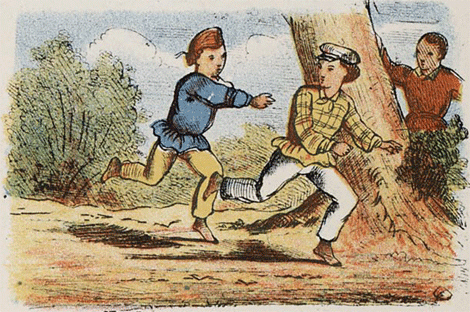
\includegraphics[width=12em]{figs/Jongensspelen_10.jpg}
  \end{center}


  \hspace*{4em}\only<2-4>{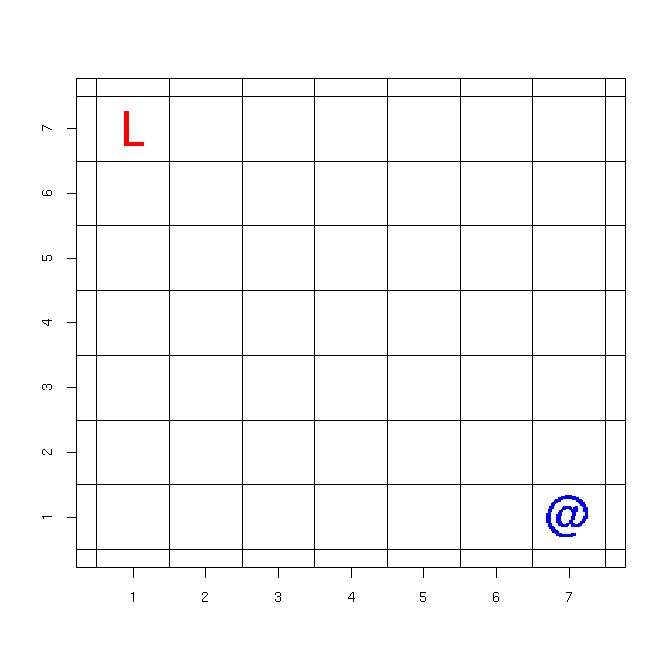
\includegraphics[width=8em]{figs/bad.png}}\quad\only<4>{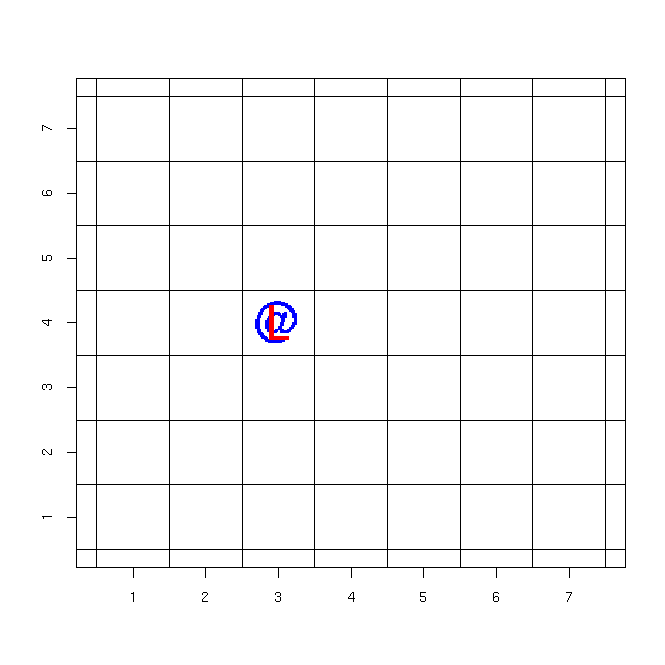
\includegraphics[width=8em]{figs/good.png}}

  \vspace*{-1em}
  \only<2-4>{\hspace*{0em} Pas bien pour le loup  $\uparrow$}
  \only<3,4>{
    \Put(-80,155){\scalebox{0.5}{
        \begin{tabular}{ccc}
          $\nwarrow$&$\uparrow$&$\nearrow$\\
          $\leftarrow$&$\cdot$&$\rightarrow$\\
          $\swarrow$&$\downarrow$&$\searrow$
        \end{tabular}
      }}
    \Put(-27.5,53.5){\scalebox{0.5}{
        \begin{tabular}{ccc}
          $\nwarrow$&$\uparrow$&$\nearrow$\\
          $\leftarrow$&$\cdot$&$\rightarrow$\\
          $\swarrow$&$\downarrow$&$\searrow$
        \end{tabular}
      }}
  }
  \vspace*{-1.5em}
  \only<4>{\hspace*{15em} $\uparrow$ Bien pour le loup}
\end{frame}


\begin{frame}[t]{Idée de l'apprentissage par renforcement}

  \centering

  \vspace{4em}
  \tikzset{
    state/.style={
      rectangle,
      rounded corners,
      draw=black, very thick,
      minimum height=10em,
      inner sep=5pt,
      text centered,
    },
  }
  

  \begin{tikzpicture}[->,>=latex, node distance = 20em]
    \node[state] (A) {Agent};

    \node[state] (E) [right of = A] {Environnement};

    \pause
    \path
    ([yshift=3em]E.west) 
    edge
    node[anchor=south,above]{état actuel}
    ([yshift=3em]A.east)
    ;

    \pause
    \path
    ([yshift=1em]A.east) 
    edge
    node[anchor=south,above]{action}
    ([yshift=1em]E.west)
    ;


    \pause
    \path
    ([yshift=-2em]E.west) 
    edge[decorate, decoration = 
    {
      snake,
      amplitude = 0.4ex,
      segment length = 1em,
      post length=0.8ex}]
    node[anchor=south,above]{récompense}
    ([yshift=-2em]A.east)
    ;

    \path
    ([yshift=-4em]E.west) 
    edge
    node[anchor=south,above]{nouvel état}
    ([yshift=-4em]A.east)
    ;
  \end{tikzpicture}

  \only<5>{
    But de l'agent : choisir les actions afin de maximiser les récompenses immediates et futures
  }

\end{frame}

\section{Historique}

\transition{Historique}

\begin{frame}{Historique}{Apprentissage par renforcement}
  \begin{itemize}
  \item[1988] TD-learning, Richard Sutton\hspace{1em}
    \raisebox{-.5\height}{%
      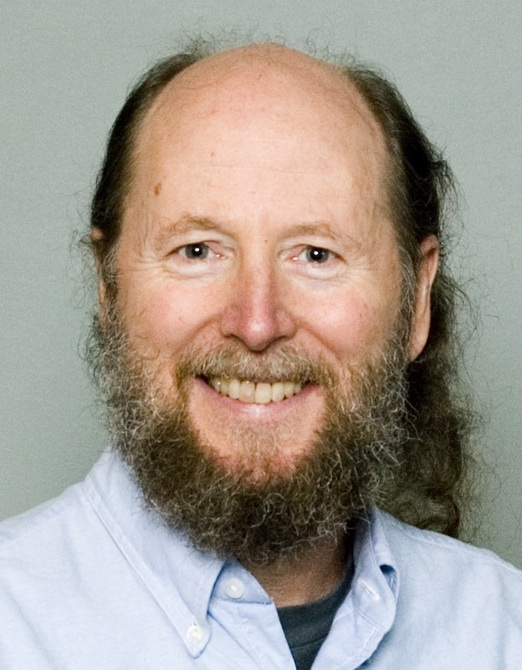
\includegraphics[width=6em]{figs/Sutton-head5.jpg}}
    
  \item[1989] Q-learning,  Chris Watkins\hspace{1.8em}
    \raisebox{-.5\height}{
      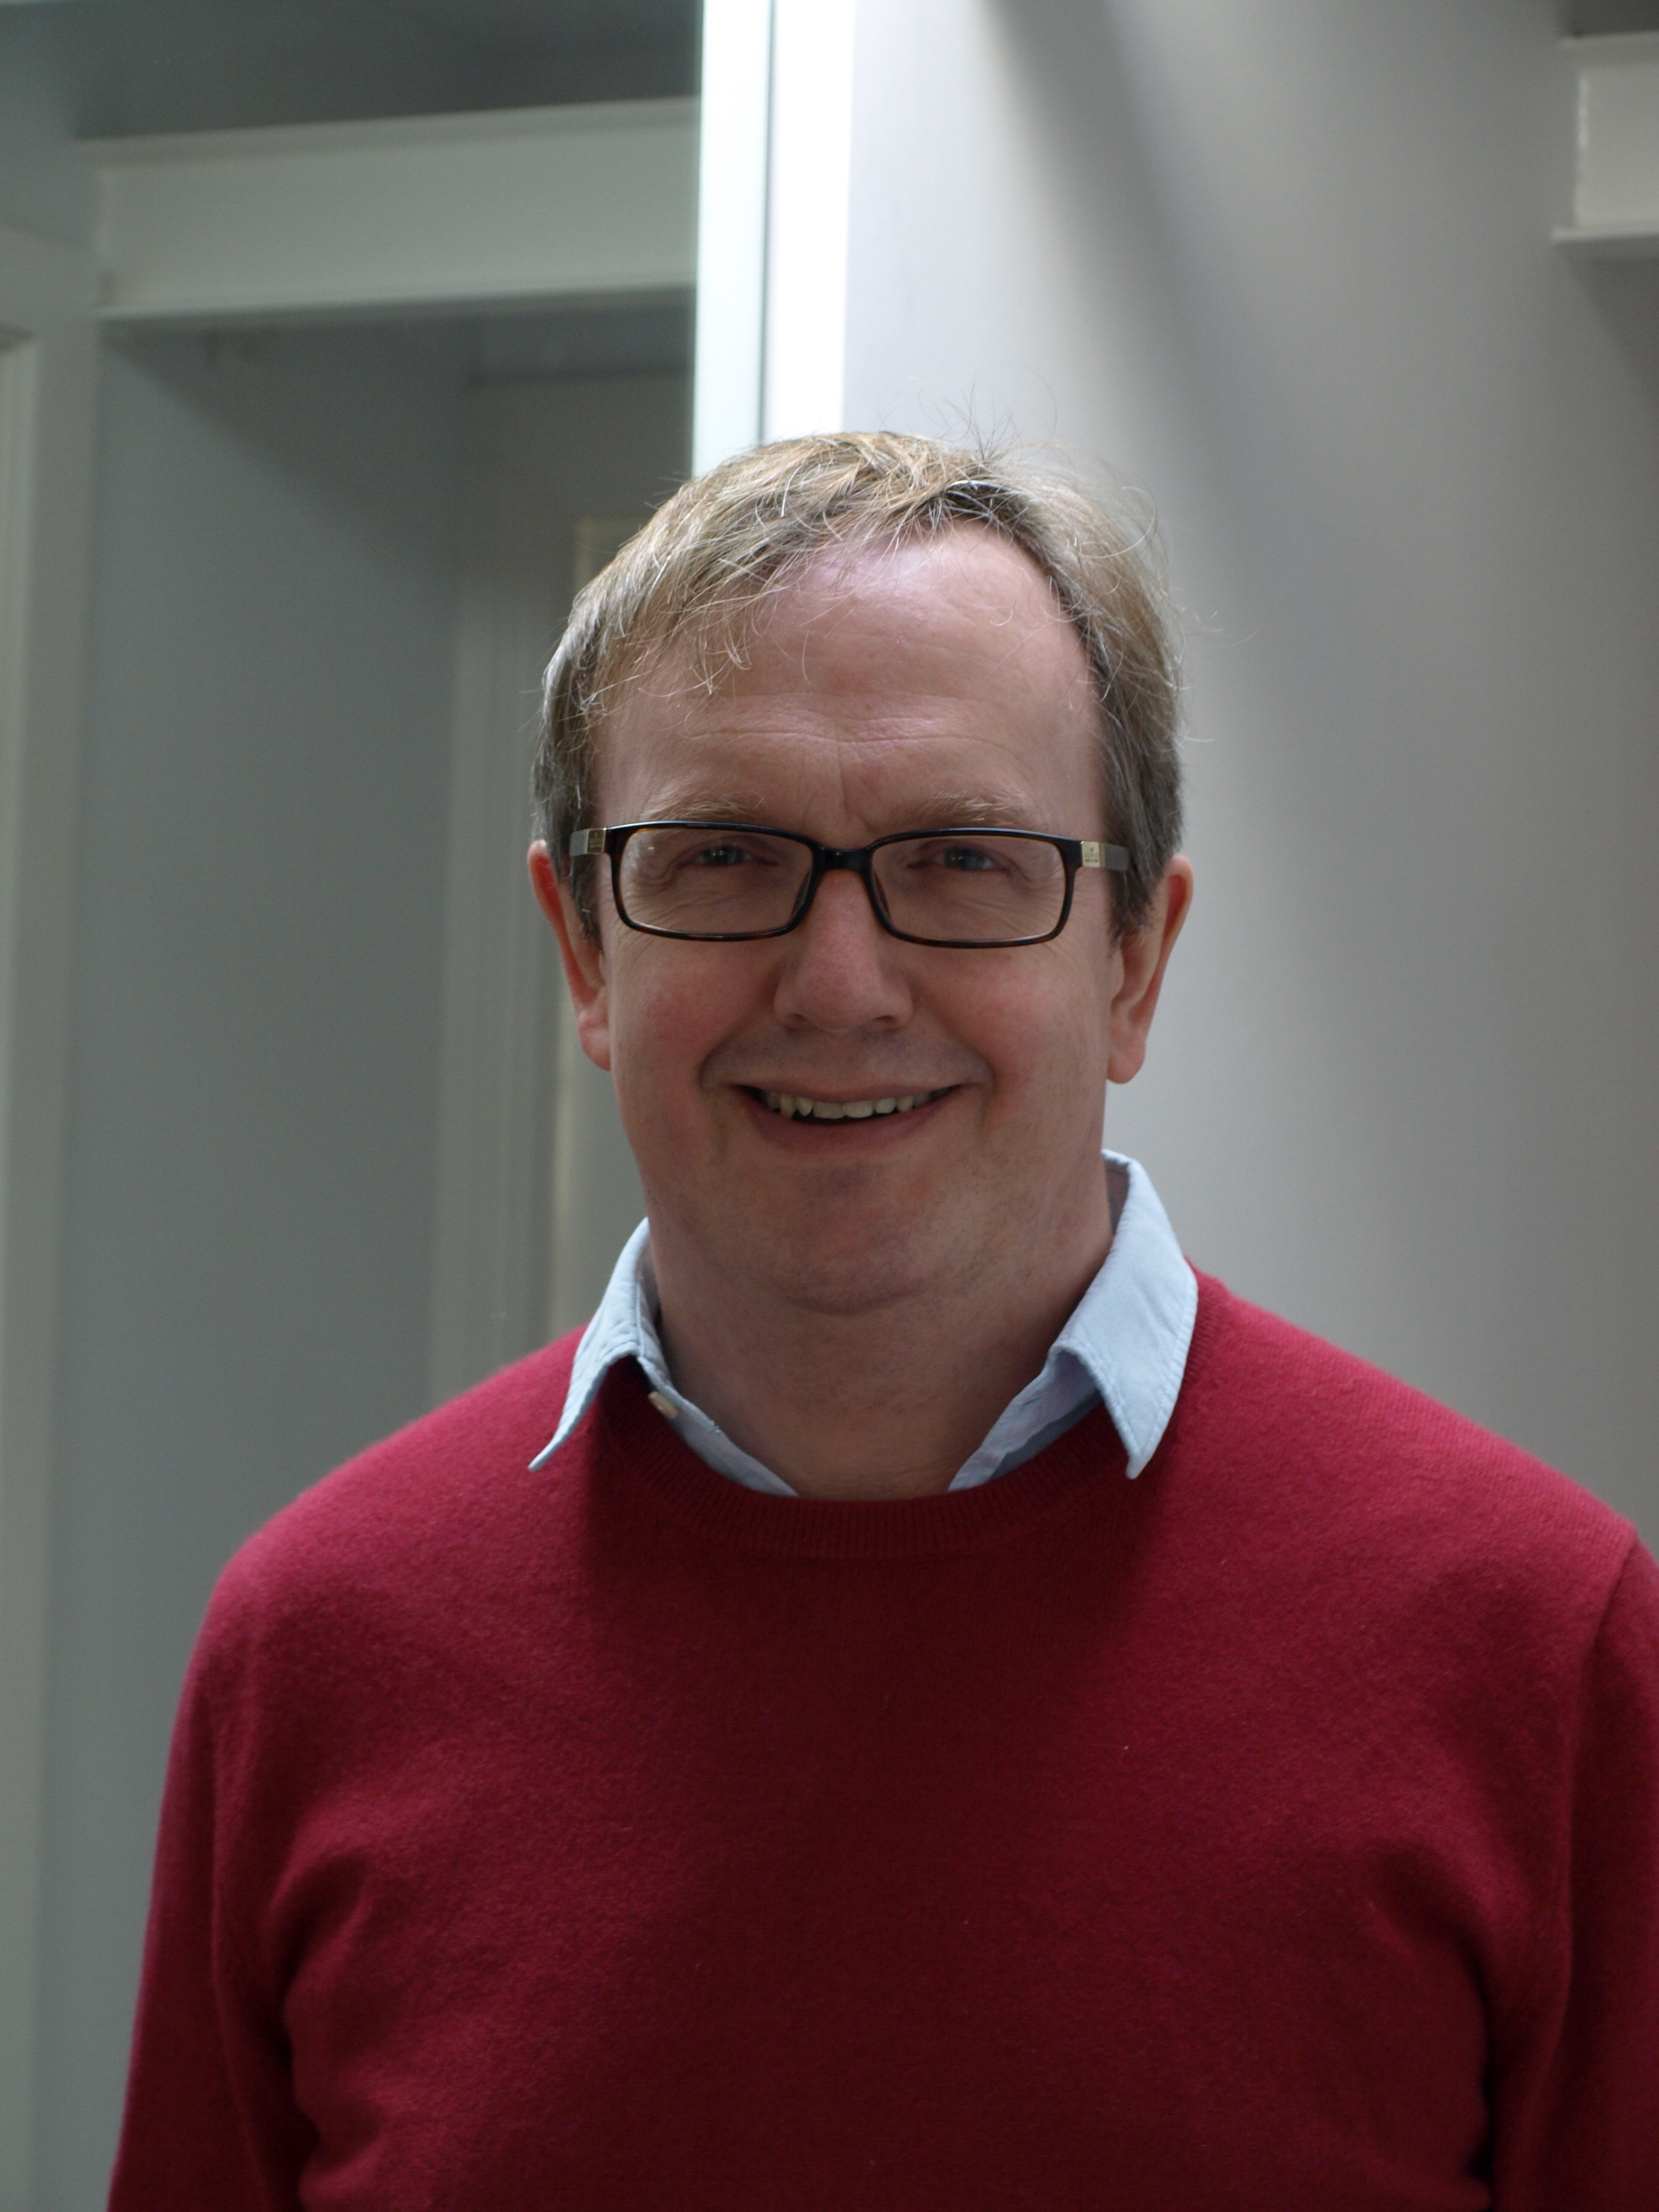
\includegraphics[width=6em]{figs/cw090311.jpg}}
    
  \end{itemize}
\end{frame}
  
\begin{frame}{Historique}

``Toutefois, l'origine de l'apprentissage par renforcement est plus
ancienne. Elle dérive de formalisations théoriques de méthodes de
contrôle optimal, visant à mettre au point un contrôleur permettant de
minimiser au cours du temps une mesure donnée du comportement d'un
système dynamique. La version discrète et stochastique de ce problème
est appelée un processus de décision markovien et fut introduite par
Richard Ernest Bellman en 1957''

\centering
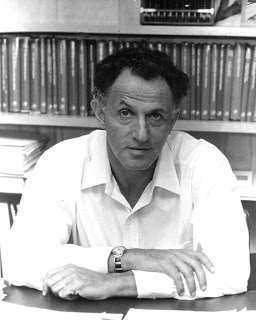
\includegraphics[width=6em]{figs/Bellman.jpg}

\hfill \scriptsize \url{https://fr.wikipedia.org/wiki/Apprentissage_par_renforcement}

\end{frame}


\begin{frame}{Théories de psychologie animale $\to$ Intelligence artificielle }
  ``D'autre part, la formalisation des problèmes d'apprentissage par
  renforcement s'est aussi beaucoup inspirée de théories de
  psychologie animale, comme celles analysant comment un animal peut
  apprendre par essais-erreurs à s'adapter à son environnement. Ces
  théories ont beaucoup inspiré le champ scientifique de
  l'intelligence artificielle et ont beaucoup contribué à l'émergence
  d'algorithmes d'apprentissage par renforcement au début des années
  1980.''

  \hfill \scriptsize --- Wikipedia
\end{frame}


\section{Théorie}
\transition{Théorie}

\begin{frame}{Livres}

\begin{enumerate}
\item {\bf Reinforcement Learning: An Introduction}

Richard S. Sutton et Andrew G. Barto

\item {\bf Processus décisionnels de Markov en intelligence artificielle}

Olivier Sigaud et  Olivier Buffet
\end{enumerate}


\begin{center}
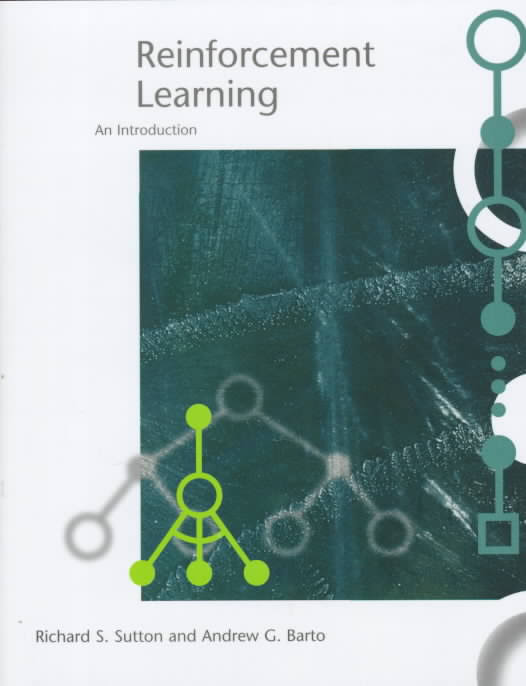
\includegraphics[width=8em]{figs/rl-book.jpeg}
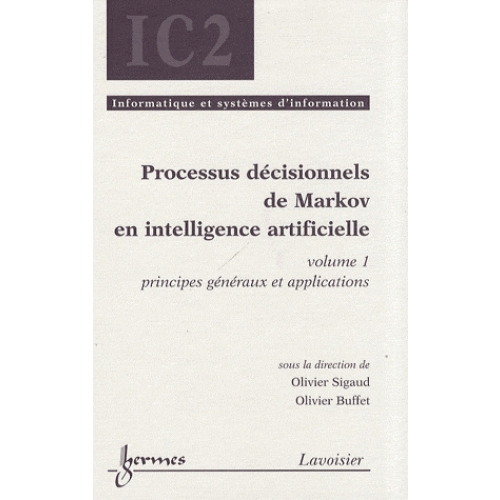
\includegraphics[width=12em]{figs/book21.jpg}
\end{center}
\end{frame}

 
\begin{frame}{Processus de décision markovien (MDP)}
  
  \begin{center}
    \tiny
    \tikzset{
      state/.style={
        rectangle,
        rounded corners,
        draw=black, very thick,
        minimum height=10em,
        inner sep=5pt,
        text centered,
      },
    }  
    \begin{tikzpicture}[->,>=latex, node distance = 20em]
      \node[state] (A) {Agent};
      
      \node[state] (E) [right of = A] {Environnement};
      
      \path
      ([yshift=3em]E.west) 
      edge
      node[anchor=south,above]{état actuel}
      ([yshift=3em]A.east)
      ;
      
      \path
      ([yshift=1em]A.east) 
      edge
      node[anchor=south,above]{action}
      ([yshift=1em]E.west)
      ;
      
      
      \path
      ([yshift=-2em]E.west) 
      edge[decorate, decoration =
      {
        snake,
        amplitude = 0.4ex,
        segment length = 1em,
        post length=0.8ex}]    
      node[anchor=south,above]{récompense}
      ([yshift=-2em]A.east)
      ;
      
      \path
      ([yshift=-4em]E.west) 
      edge
      node[anchor=south,above]{nouvel état}
      ([yshift=-4em]A.east)
      ;
    \end{tikzpicture}

    But de l'agent : choisir les actions afin de maximiser les récompenses immediates et futures
  \end{center}

  \begin{block}{Definitions}
    \begin{itemize}
    \item $S$ --- ensemble d'états
    \item $A$ --- ensemble d'actions
    \item $\Pr [s'|s,a]$ --- probabilité de se retrouver dans l'état
      $s'$ en faisant l'action $a$ dans l'état $s$ (probabilité de
      transition)
    \item $R : S \times A \times S \to \R$ --- fonction de récompense
    \item $\pi : S \to A$ --- politique de l'agent
    \end{itemize}
  \end{block}


\end{frame}


\begin{frame}[fragile]{Processus de décision markovien (MDP)}

  {
    \scriptsize
    \begin{block}{Definitions}
      \begin{itemize}
      \item $S$ --- ensemble d'états
      \item $A$ --- ensemble d'actions
      \item $\Pr [s'|s,a]$ --- probabilité de se retrouver dans l'état $s'$ en
        faisant l'action $a$ dans l'état $s$ (probabilité de transition)
      \item $R : S \times A \times S \to \R$ --- fonction de récompense
      \item $\pi : S \to A$ --- politique de l'agent
      \end{itemize}
    \end{block}
  }

  \vspace{-1ex}
  \begin{block}{Processus}
    \vspace{-1.5em}
    \small
    $$\begin{tikzcd}[column sep = small,
      decoration =
      {
        snake,
        amplitude = 0.2ex,
        segment length = 0.3em,
        post length=0.8ex}]
      s_0 \arrow{rr}{\pi(s_0)} &\arrow[decorate]{d}&
      s_1 \arrow{rr}{\pi(s_1)} &\arrow[decorate]{d}&
      s_2 \arrow{rr}{\pi(s_2)} &\arrow[decorate]{d}&
      s_3 \arrow{rr}{\pi(s_3)} &\arrow[decorate]{d}& \cdots \\
      & r_0 && r_1  && r_2 && r_3 \\
    \end{tikzcd}
    $$
  \end{block}
  \vspace{-2.5em}

  $s_n$ --- état à la $n$-ième iteration

  $r_n$ --- $n$-ième récompense
  
  Bonne politique maximise  $\E \sum_{n = 0}^\infty \gamma^n r_n$, $0 < \gamma < 1$
  

\end{frame}

\begin{frame}[t]{Q-learning}

  Bonne politique maximise l'espérance de $\sum_{n = 0}^\infty \gamma^n r_n$
  \vspace{2em}

  {\bf Comment trouver cette politique ?} 

  Par exemple, par l'algorithme Q-learning.
  
  \begin{definition}
    \begin{itemize}
    \item  $Q : S \times A \to \R$ --- fonction qualité de l'action 
    \item  $\pi (s) = \argmax_{a \in A} Q(s, a)$
    \end{itemize}
  \end{definition}
  
  \vspace{-1em}
  \begin{block}{Algorithm}
    {\bf Initialisation:} $\forall s \in S, a \in A  \quad Q_0 (s,a) \leftarrow 0$
    \vspace{1em}

    {\bf Règle de mise à jour:}
    \vspace{-1em}\begin{multline*}
      Q_{n+1}(s_n,a_n) \leftarrow (1 - \alpha_n) \cdot Q_n(s_n,a_n)  + \\
      \alpha_n \cdot \left( r_n + \gamma \max_a Q_n(s_{n+1},a)     \right)
    \end{multline*}
  \end{block}

\end{frame}


%% TODO: EXPLIKE O TABLO ADD LES SLIDES
%% keske space si alpha_n = 1 (determinist processus) 
%% keske space si alpha_n = 0 (Q change pas)
%% moyen iterativ http://www.heikohoffmann.de/htmlthesis/node134.html

\begin{frame}[t]{Convergence}

  {
    \scriptsize
    \begin{block}{Algorithm}
      $ Q_{n+1}(s_n,a_n) \leftarrow Q_n(s_n,a_n) (1 - \alpha_n) +
        \alpha_n \left( r_n + \gamma \max_a Q_n(s_{n+1},a)     \right)$
    \end{block}
  }
  

  
  \only<1>{
    \begin{block}{Optimum}
      $\mathfrak{Q}$ --- ensemble de fonctions de type $S \times A \to \R$.
      
      $Q^* \in \mathfrak{Q}$ est une fonction t.q. $\forall Q \in
      \mathfrak{Q}, s \in S, a \in A$ on a $Q(s,a) \le Q^* (s,a)$
    \end{block}
    \vspace{1em}      

    {\em 
      On peut prouver l'existence de $Q^*$ en utilisant le théorème de
      point fixe de Banach.
    }
  }

  \only<2> {  
    \begin{block}{Théorème}
      $Q_n$ converge presque sûrement vers $Q^*$ si :
      \begin{enumerate}
      \item $A$ et $S$ sont finis
      \item les probabilites de transitions ne changent pas
      \item l'agent essaie chaque action dans chaque état un nombre infini de fois
      \item $\sum_{n=0} \alpha_n = \infty$ et $\sum_{n=0}^\infty \alpha_n^2 < \infty$
      \item $\gamma < 1$
      \end{enumerate}
    \end{block}
    
    \vspace{1ex}
    
    {\em
    La preuve est basée sur les idées des algorithmes itératives
    d'optimisation stochastiques des années 1950 (algorithms de
    Robbins-Monro, Kiefer-Wolfowitz, etc) }
}

\end{frame}


\begin{frame}{Exploration de l'environnement}
  
  \centering

  Il faut agir et apprendre

  \begin{block}{Alors,}
    \begin{itemize}
    \item parfois l'agent utilise $Q$ : $\pi (s) = \argmax_{a \in A} Q(s, a)$
    \item parfois il agit au hasard : $\pi (s) = \rand (a \in A) $
    \end{itemize}
  \end{block}


\end{frame}


\begin{frame}{Quelques remarques}

  \begin{block}{Algorithm}
    \scriptsize
    $ Q_{n+1}(s_n,a_n) \leftarrow Q_n(s_n,a_n) (1 - \alpha_n) +
    \alpha_n \left( r_n + \gamma \max_a Q_n(s_{n+1},a)     \right)$
  \end{block}  

  \vspace{2em}

  Dans la vie réelle les probabilites de transitions ne sont pas
  nécessairement fixes.  Il faut apprendre toujours et donc $\alpha_n$
  peut être constante.

  \vspace{2em}


  Vitesse d'apprentissage est caractéristique très importante.

  
\end{frame}



\section{Applications}

\transition{Applications et recherche actuelle}

% Thus, reinforcement learning is particularly well suited to problems
% which include a long-term versus short-term reward trade-off. It has
% been applied successfully to various problems, including robot
% control, elevator scheduling, telecommunications, backgammon,
% checkers (Sutton \& Barto 1998, Chapter 11) and go (AlphaGo).


\begin{frame}{AlphaGo}
  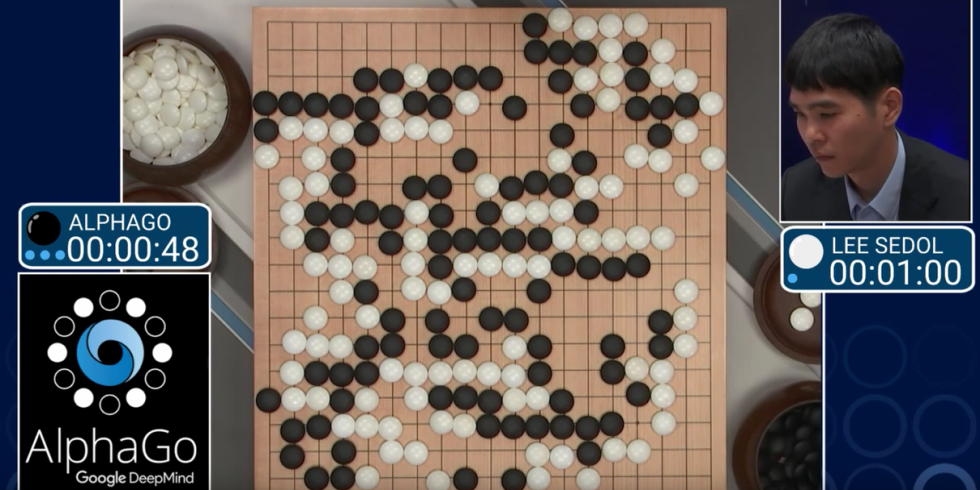
\includegraphics[width=\textwidth]{figs/alphago.png}

  \vspace{1ex}

  ``This program was based on general-purpose AI methods {\bf
    [including reinforcement learning]}, using deep neural networks to
  mimic expert players, and further improving the program by learning
  from games played against itself.''

  \hfill \scriptsize --- \url{https://deepmind.com/research/alphago}
\end{frame}


\begin{frame}{Allocation des ressources dans le cloud}
  
\includegraphics[width=\textwidth]{figs/mypaper.png}
\end{frame}


\begin{frame}{Neurobiologie}

  \begin{center}
    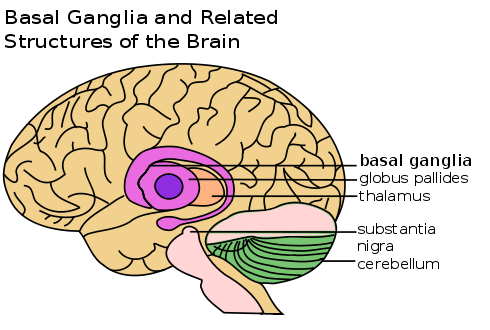
\includegraphics[width=12em]{figs/ganglions-de-base.png}
  \end{center}

  ``La collaboration entre neurobiologistes et chercheurs en
  intelligence artificielle a permis de découvrir qu'une partie du
  cerveau fonctionnait de façon très similaire aux algorithmes
  d'apprentissage par renforcement.'' 

  \hfill \scriptsize --- Wikipedia

  \vspace{1em}

  {\bf A Model of How the Basal Ganglia Generate and Use Neural Signals that Predict Reinforcement}  \\
  \hfill James C. Houk,  J. L. Adams, A. G. Barto



\end{frame}

\section{Recherche actuelle}

\begin{frame}{Recherche actuelle et future}

\begin{itemize}
\item Environnements sont plus grands
\item Il faut augmenter la vitesse de convergence
\item Combinaison avec d'autres techniques d'apprentissage par machine
  (les réseaux de neurones, etc)
\end{itemize}
\end{frame}

% Le raffinement actuel des algorithmes d'apprentissage par
% renforcement inspire les travaux des neurobiologistes et des
% psychologues pour la compréhension du fonctionnement du cerveau et
% du comportement animal.

% tels que le TD-learning. Il semblerait ainsi que la nature ait
% découvert, au fil de l'évolution, une façon semblable à celles
% trouvées par des chercheurs pour optimiser la façon dont un agent ou
% organisme peut apprendre par essais-erreurs. Ou plutôt, les chercheurs
% en intelligence artificielle ont redécouvert en partie ce que la
% nature avait mis des millions d'années à mettre en place.

\section{TP : Jeu du loup en R}

\transition{En TP : Jeu du loup en R}

\begin{frame}[t]{Jeu du loup}{en R}
  \begin{center}
    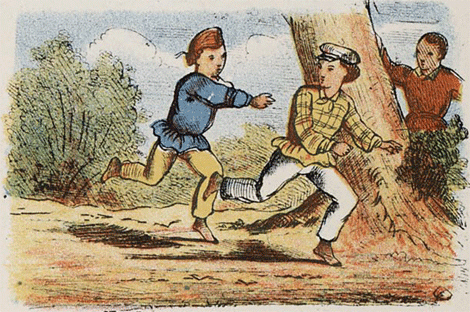
\includegraphics[width=6em]{figs/Jongensspelen_10.jpg}
  \end{center}

  Code source: \url{https://github.com/kerzol/jeu-du-loup}

  \vspace{2em}

  \hspace*{4em}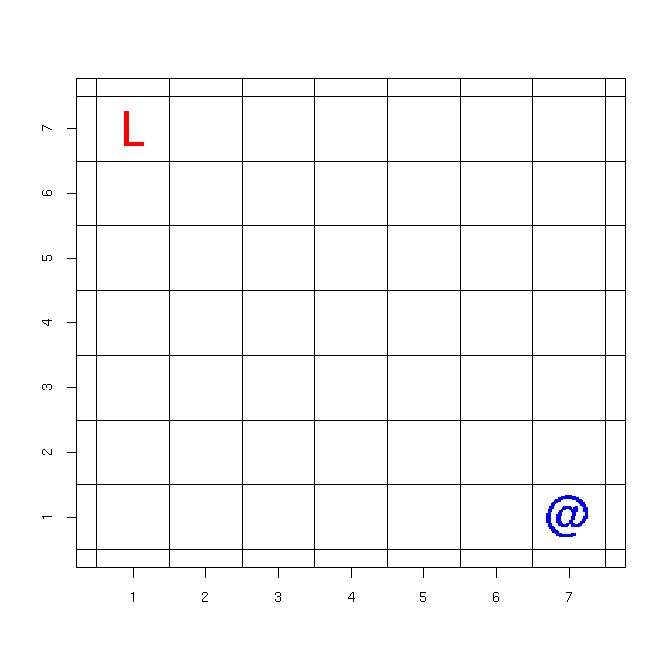
\includegraphics[width=8em]{figs/bad.png}\quad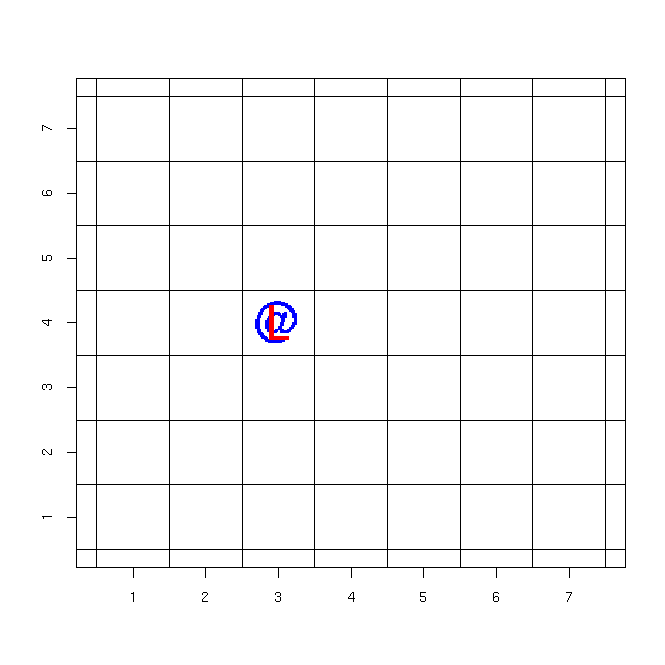
\includegraphics[width=8em]{figs/good.png}

  \vspace*{-1em}
  \hspace*{0em} Pas bien pour le loup  $\uparrow$ 
  \Put(-76.5,156){\scalebox{0.5}{
      \begin{tabular}{ccc}
        $\nwarrow$&$\uparrow$&$\nearrow$\\
        $\leftarrow$&$\cdot$&$\rightarrow$\\
        $\swarrow$&$\downarrow$&$\searrow$
      \end{tabular}
    }}
  \Put(-23.5,53.5){\scalebox{0.5}{
      \begin{tabular}{ccc}
        $\nwarrow$&$\uparrow$&$\nearrow$\\
        $\leftarrow$&$\cdot$&$\rightarrow$\\
        $\swarrow$&$\downarrow$&$\searrow$
      \end{tabular}
    }}
  
  \vspace*{-1.5em}
  \hspace*{15em} $\uparrow$ Bien pour le loup



\end{frame}


\begin{frame}{En TP / Devoir à la maison}

  \begin{enumerate}
  \item Télécharger le code source : \url{https://github.com/kerzol/jeu-du-loup}
  \item Lire le code, comprendre le code
  \item Trouvez et décrire les différences entre {\tt q-loup.R} et {\tt q-loup-1.R}
  \item Pourquoi {\tt q-loup-1.R} apprend mieux le comportement cyclique du chat ?
  \item Visualisez l'evolution de valeurs de $Q$
  \item Change {\tt ALPHA = 0.6} dans le code par quelque chose qui
    respecte la condition $\sum_{n=0}^\infty \alpha_n < \infty$
  \item Ajouter quelques murs dans l'environnement.
  \end{enumerate}
\end{frame}



\transition{Merci}

\end{document}

